\documentclass[10pt,twocolumn,letterpaper]{article}
\usepackage[pagenumbers]{cvpr}
\usepackage{hyperref}

% ── Additional packages (cvpr.sty already loads: times, xcolor, graphicx,
%    amsmath, amssymb, booktabs, caption, subcaption) ──
\usepackage{tikz}
\usepackage{pgfplots}
\pgfplotsset{compat=1.18}
\usetikzlibrary{
  arrows.meta,
  calc,
  positioning,
  shapes.geometric,
  fit,
  backgrounds,
  matrix
}
\usepackage{float}

% ── Colors ──
\definecolor{dinoblue}{RGB}{41,98,168}
\definecolor{rgbgreen}{RGB}{34,139,34}
\definecolor{thermalred}{RGB}{178,34,34}
\definecolor{blockblue}{RGB}{220,235,252}
\definecolor{blockred}{RGB}{252,225,220}
\definecolor{blockgreen}{RGB}{220,252,225}
\definecolor{blockgray}{RGB}{240,240,240}

% ── Macros ──
\newcommand{\cls}{\texttt{[CLS]}}

\begin{document}

% ══════════════════════════════════════════════════════════════
%  TITLE
% ══════════════════════════════════════════════════════════════
\title{Municipal Waste Classification with DINOv2 Embeddings:\\RGB and Thermal Pipeline Performance}

\author{%
}

\maketitle

% ══════════════════════════════════════════════════════════════
%  ABSTRACT
% ══════════════════════════════════════════════════════════════
\begin{abstract}
We present two single-modal classification pipelines for automated conveyor belt waste sorting into four material classes (glass, metal, paper, plastic) using a frozen DINOv2 ViT-L/14 backbone. Each pipeline trains only a lightweight attention pooling layer and MLP classification head (${\sim}$528K parameters, 0.17\% of the backbone), operating on pre-cached \cls{} token features. Evaluated via 5-fold stratified cross-validation on 550 labeled tracklets from 19 experiment videos, the RGB pipeline achieves \textbf{95.1\%} macro F1 (27 errors) while the thermal pipeline achieves \textbf{90.6\%} macro F1 (48 errors). Glass is near-perfectly classified in both modalities (F1 $\geq$ 0.97), while paper remains the most challenging class, particularly for thermal (F1 = 0.804). The thermal modality, despite lower standalone accuracy, captures complementary material properties that benefit downstream fusion.
\end{abstract}

% ══════════════════════════════════════════════════════════════
%  1  INTRODUCTION
% ══════════════════════════════════════════════════════════════
\section{Introduction}

This report summarizes the performance of two single-modal classification pipelines for conveyor belt waste sorting into four material classes: \textbf{glass}, \textbf{metal}, \textbf{paper}, and \textbf{plastic}. Both pipelines use a frozen DINOv2 ViT-L/14 backbone (${\sim}$304M parameters) as a feature extractor, with only a lightweight attention pooling layer and MLP classification head trained (${\sim}$528K trainable parameters each, 0.17\% of backbone). All results are from \textbf{5-fold stratified cross-validation} on 550 labeled tracklets from 19 experiment videos.


% ══════════════════════════════════════════════════════════════
%  2  RGB PIPELINE
% ══════════════════════════════════════════════════════════════
\section{RGB Pipeline}

\subsection{Architecture}

\begin{figure}[t]
\centering
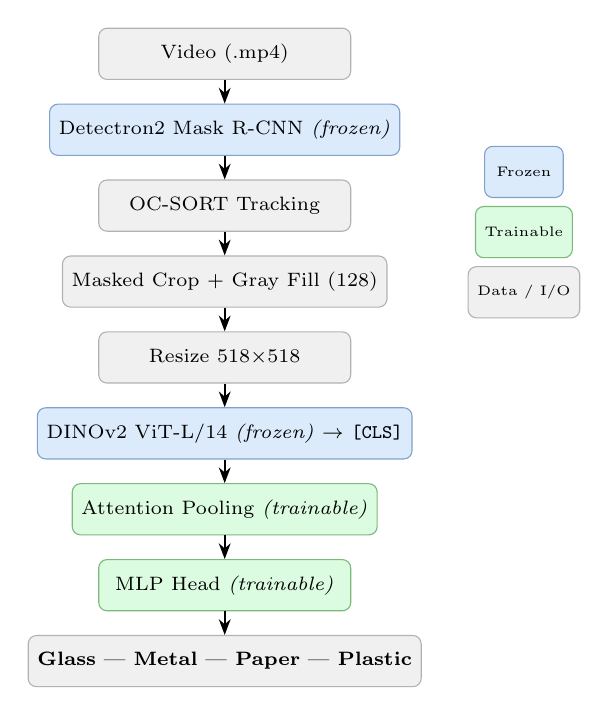
\begin{tikzpicture}[
  block/.style={draw, rounded corners=3pt, minimum height=0.65cm,
                minimum width=3.2cm, align=center, font=\scriptsize},
  frozen/.style={block, fill=blockblue, draw=dinoblue!60},
  train/.style={block, fill=blockgreen, draw=rgbgreen!60},
  data/.style={block, fill=blockgray, draw=black!30},
  arr/.style={-{Stealth[length=2mm]}, semithick},
  node distance=0.3cm
]

\node[data] (video) {Video (.mp4)};
\node[frozen, below=of video] (det) {Detectron2 Mask R-CNN \textit{(frozen)}};
\node[data, below=of det] (track) {OC-SORT Tracking};
\node[data, below=of track] (mask) {Masked Crop + Gray Fill (128)};
\node[data, below=of mask] (resize) {Resize 518$\times$518};
\node[frozen, below=of resize] (dino) {DINOv2 ViT-L/14 \textit{(frozen)} $\to$ \cls{}};
\node[train, below=of dino] (pool) {Attention Pooling \textit{(trainable)}};
\node[train, below=of pool] (head) {MLP Head \textit{(trainable)}};
\node[data, below=of head] (out) {\textbf{Glass} | \textbf{Metal} | \textbf{Paper} | \textbf{Plastic}};

\draw[arr] (video) -- (det);
\draw[arr] (det) -- (track);
\draw[arr] (track) -- (mask);
\draw[arr] (mask) -- (resize);
\draw[arr] (resize) -- (dino);
\draw[arr] (dino) -- (pool);
\draw[arr] (pool) -- (head);
\draw[arr] (head) -- (out);

% Legend
\node[frozen, minimum width=1cm, font=\tiny] at (3.8, -1.5) (leg1) {Frozen};
\node[train, minimum width=1cm, font=\tiny, below=0.1cm of leg1] (leg2) {Trainable};
\node[data, minimum width=1cm, font=\tiny, below=0.1cm of leg2] (leg3) {Data / I/O};

\end{tikzpicture}
\caption{RGB classification pipeline. Detection and DINOv2 are frozen; only the attention pool and MLP head are trained (${\sim}$528K parameters).}
\label{fig:rgb_pipeline}
\end{figure}

The RGB pipeline (Fig.~\ref{fig:rgb_pipeline}) processes video through a frozen Detectron2 Mask R-CNN detector and OC-SORT multi-object tracker. Per-tracklet masked crops (gray fill 128, resized to 518$\times$518) are passed through a frozen DINOv2 ViT-L/14 to extract \cls{} token features. A trainable attention pooling layer aggregates 8 uniformly sampled frame features into a single tracklet representation, classified by an MLP head.

\subsection{Results}

\begin{table}[t]
\centering
\caption{RGB pipeline: 5-fold stratified CV (550 tracklets).}
\label{tab:rgb_overall}
\begin{tabular}{@{}lc@{}}
\toprule
\textbf{Metric} & \textbf{Value} \\
\midrule
Mean Accuracy & $0.9509 \pm 0.0093$ \\
Mean Macro F1 & $0.9507 \pm 0.0110$ \\
Pooled Accuracy & $0.9509$ \\
Total Errors & 27 / 550 \\
\bottomrule
\end{tabular}
\end{table}

\begin{table}[t]
\centering
\caption{RGB per-class metrics (pooled across all 5 folds).}
\label{tab:rgb_perclass}
\begin{tabular}{@{}lcccc@{}}
\toprule
\textbf{Class} & \textbf{Prec.} & \textbf{Rec.} & \textbf{F1} & \textbf{N} \\
\midrule
Glass   & 0.978 & 0.992 & 0.985 & 132 \\
Metal   & 0.921 & 0.977 & 0.948 & 131 \\
Paper   & 0.957 & 0.908 & 0.932 & 98 \\
Plastic & 0.951 & 0.926 & 0.938 & 189 \\
\bottomrule
\end{tabular}
\end{table}

Tables~\ref{tab:rgb_overall} and~\ref{tab:rgb_perclass} summarize the RGB results. The pipeline achieves 95.1\% macro F1 with only 27 errors across 550 tracklets. Glass is near-perfect (F1=0.985), while paper and plastic show the most room for improvement.

\subsection{Confusion Matrix}

\begin{figure}[t]
\centering
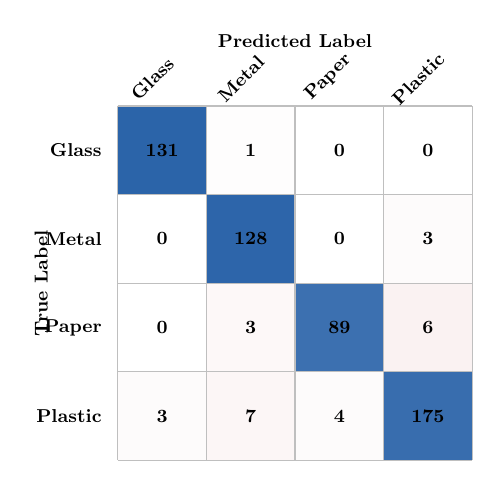
\begin{tikzpicture}[font=\scriptsize, scale=0.75, every node/.style={scale=0.75}]
  % Row 0: Glass  (131, 1, 0, 0)
  \fill[dinoblue!99!white] (0, 0) rectangle (1.5, 1.5);
  \fill[thermalred!1!white] (1.5, 0) rectangle (3, 1.5);
  \fill[white] (3, 0) rectangle (4.5, 1.5);
  \fill[white] (4.5, 0) rectangle (6, 1.5);
  % Row 1: Metal  (0, 128, 0, 3)
  \fill[white] (0, -1.5) rectangle (1.5, 0);
  \fill[dinoblue!98!white] (1.5, -1.5) rectangle (3, 0);
  \fill[white] (3, -1.5) rectangle (4.5, 0);
  \fill[thermalred!2!white] (4.5, -1.5) rectangle (6, 0);
  % Row 2: Paper  (0, 3, 89, 6)
  \fill[white] (0, -3) rectangle (1.5, -1.5);
  \fill[thermalred!3!white] (1.5, -3) rectangle (3, -1.5);
  \fill[dinoblue!91!white] (3, -3) rectangle (4.5, -1.5);
  \fill[thermalred!6!white] (4.5, -3) rectangle (6, -1.5);
  % Row 3: Plastic  (3, 7, 4, 175)
  \fill[thermalred!2!white] (0, -4.5) rectangle (1.5, -3);
  \fill[thermalred!4!white] (1.5, -4.5) rectangle (3, -3);
  \fill[thermalred!2!white] (3, -4.5) rectangle (4.5, -3);
  \fill[dinoblue!93!white] (4.5, -4.5) rectangle (6, -3);

  % Grid
  \foreach \i in {0,...,4} {
    \draw[gray!50] (\i*1.5, 1.5) -- (\i*1.5, -4.5);
    \draw[gray!50] (0, 1.5-\i*1.5) -- (6, 1.5-\i*1.5);
  }

  % Values
  \node[font=\small\bfseries] at (0.75, 0.75) {131};
  \node[font=\small\bfseries] at (2.25, 0.75) {1};
  \node[font=\small\bfseries] at (3.75, 0.75) {0};
  \node[font=\small\bfseries] at (5.25, 0.75) {0};
  \node[font=\small\bfseries] at (0.75, -0.75) {0};
  \node[font=\small\bfseries] at (2.25, -0.75) {128};
  \node[font=\small\bfseries] at (3.75, -0.75) {0};
  \node[font=\small\bfseries] at (5.25, -0.75) {3};
  \node[font=\small\bfseries] at (0.75, -2.25) {0};
  \node[font=\small\bfseries] at (2.25, -2.25) {3};
  \node[font=\small\bfseries] at (3.75, -2.25) {89};
  \node[font=\small\bfseries] at (5.25, -2.25) {6};
  \node[font=\small\bfseries] at (0.75, -3.75) {3};
  \node[font=\small\bfseries] at (2.25, -3.75) {7};
  \node[font=\small\bfseries] at (3.75, -3.75) {4};
  \node[font=\small\bfseries] at (5.25, -3.75) {175};

  % Column labels
  \node[font=\small\bfseries, rotate=45, anchor=south] at (0.75, 1.8) {Glass};
  \node[font=\small\bfseries, rotate=45, anchor=south] at (2.25, 1.8) {Metal};
  \node[font=\small\bfseries, rotate=45, anchor=south] at (3.75, 1.8) {Paper};
  \node[font=\small\bfseries, rotate=45, anchor=south] at (5.25, 1.8) {Plastic};

  % Row labels
  \node[font=\small\bfseries, anchor=east] at (-0.15, 0.75) {Glass};
  \node[font=\small\bfseries, anchor=east] at (-0.15, -0.75) {Metal};
  \node[font=\small\bfseries, anchor=east] at (-0.15, -2.25) {Paper};
  \node[font=\small\bfseries, anchor=east] at (-0.15, -3.75) {Plastic};

  \node[font=\small\bfseries, rotate=90] at (-1.3, -1.5) {True Label};
  \node[font=\small\bfseries] at (3, 2.6) {Predicted Label};
\end{tikzpicture}
\caption{RGB confusion matrix (pooled, 5 folds). 27 errors; glass near-perfect (131/132). Most confusion: plastic$\leftrightarrow$metal (10) and paper$\leftrightarrow$plastic (10).}
\label{fig:rgb_confusion}
\end{figure}

The confusion matrix (Fig.~\ref{fig:rgb_confusion}) reveals that glass is nearly perfectly classified (131/132). Most errors involve plastic confused with metal (7+3=10 errors) and paper confused with plastic (6+4=10 errors), reflecting visual similarity between these materials.


% ══════════════════════════════════════════════════════════════
%  3  THERMAL PIPELINE
% ══════════════════════════════════════════════════════════════
\section{Thermal Pipeline}

\subsection{Architecture}

\begin{figure}[t]
\centering
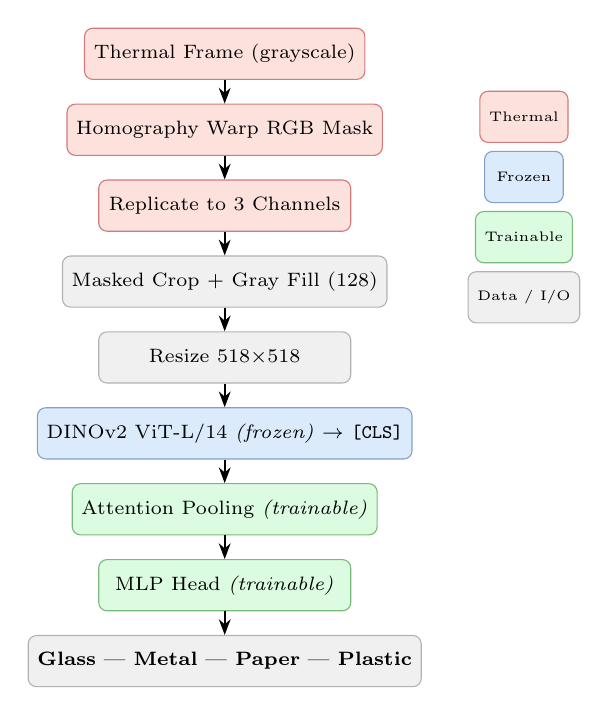
\begin{tikzpicture}[
  block/.style={draw, rounded corners=3pt, minimum height=0.65cm,
                minimum width=3.2cm, align=center, font=\scriptsize},
  frozen/.style={block, fill=blockblue, draw=dinoblue!60},
  train/.style={block, fill=blockgreen, draw=rgbgreen!60},
  data/.style={block, fill=blockgray, draw=black!30},
  thermal/.style={block, fill=blockred, draw=thermalred!60},
  arr/.style={-{Stealth[length=2mm]}, semithick},
  node distance=0.3cm
]

\node[thermal] (frame) {Thermal Frame (grayscale)};
\node[thermal, below=of frame] (warp) {Homography Warp RGB Mask};
\node[thermal, below=of warp] (rep) {Replicate to 3 Channels};
\node[data, below=of rep] (mask) {Masked Crop + Gray Fill (128)};
\node[data, below=of mask] (resize) {Resize 518$\times$518};
\node[frozen, below=of resize] (dino) {DINOv2 ViT-L/14 \textit{(frozen)} $\to$ \cls{}};
\node[train, below=of dino] (pool) {Attention Pooling \textit{(trainable)}};
\node[train, below=of pool] (head) {MLP Head \textit{(trainable)}};
\node[data, below=of head] (out) {\textbf{Glass} | \textbf{Metal} | \textbf{Paper} | \textbf{Plastic}};

\draw[arr] (frame) -- (warp);
\draw[arr] (warp) -- (rep);
\draw[arr] (rep) -- (mask);
\draw[arr] (mask) -- (resize);
\draw[arr] (resize) -- (dino);
\draw[arr] (dino) -- (pool);
\draw[arr] (pool) -- (head);
\draw[arr] (head) -- (out);

% Legend
\node[thermal, minimum width=1cm, font=\tiny] at (3.8, -0.8) (leg0) {Thermal};
\node[frozen, minimum width=1cm, font=\tiny, below=0.1cm of leg0] (leg1) {Frozen};
\node[train, minimum width=1cm, font=\tiny, below=0.1cm of leg1] (leg2) {Trainable};
\node[data, minimum width=1cm, font=\tiny, below=0.1cm of leg2] (leg3) {Data / I/O};

\end{tikzpicture}
\caption{Thermal classification pipeline. Red blocks indicate thermal-specific steps: homography-based mask warping and grayscale-to-3-channel replication.}
\label{fig:thermal_pipeline}
\end{figure}

The thermal pipeline (Fig.~\ref{fig:thermal_pipeline}) reuses the same tracklet detection and tracking from the RGB pipeline but extracts features from thermal frames instead. RGB-space masks are warped to thermal coordinates via a per-experiment homography matrix, and single-channel grayscale thermal images are replicated to 3 channels for DINOv2 compatibility.

\subsection{Results}

\begin{table}[t]
\centering
\caption{Thermal pipeline: 5-fold stratified CV (550 tracklets).}
\label{tab:thermal_overall}
\begin{tabular}{@{}lc@{}}
\toprule
\textbf{Metric} & \textbf{Value} \\
\midrule
Mean Accuracy & $0.9127 \pm 0.0384$ \\
Mean Macro F1 & $0.9056 \pm 0.0405$ \\
Pooled Accuracy & $0.9127$ \\
Total Errors & 48 / 550 \\
\bottomrule
\end{tabular}
\end{table}

\begin{table}[t]
\centering
\caption{Thermal per-class metrics (pooled across all 5 folds).}
\label{tab:thermal_perclass}
\begin{tabular}{@{}lcccc@{}}
\toprule
\textbf{Class} & \textbf{Prec.} & \textbf{Rec.} & \textbf{F1} & \textbf{N} \\
\midrule
Glass   & 0.956 & 0.985 & 0.970 & 132 \\
Metal   & 0.938 & 0.924 & 0.931 & 131 \\
Paper   & 0.792 & 0.816 & 0.804 & 98 \\
Plastic & 0.929 & 0.905 & 0.917 & 189 \\
\bottomrule
\end{tabular}
\end{table}

Tables~\ref{tab:thermal_overall} and~\ref{tab:thermal_perclass} show that the thermal pipeline achieves 90.6\% macro F1 with 48 errors. Glass remains strong (F1=0.970), but paper drops significantly to F1=0.804, reflecting similar thermal signatures between paper and plastic materials.

\subsection{Confusion Matrix}

\begin{figure}[t]
\centering
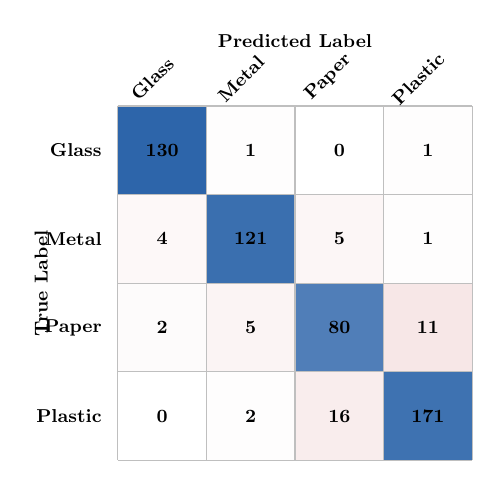
\begin{tikzpicture}[font=\scriptsize, scale=0.75, every node/.style={scale=0.75}]
  % Row 0: Glass  (130, 1, 0, 1)
  \fill[dinoblue!98!white] (0, 0) rectangle (1.5, 1.5);
  \fill[thermalred!1!white] (1.5, 0) rectangle (3, 1.5);
  \fill[white] (3, 0) rectangle (4.5, 1.5);
  \fill[thermalred!1!white] (4.5, 0) rectangle (6, 1.5);
  % Row 1: Metal  (4, 121, 5, 1)
  \fill[thermalred!3!white] (0, -1.5) rectangle (1.5, 0);
  \fill[dinoblue!92!white] (1.5, -1.5) rectangle (3, 0);
  \fill[thermalred!4!white] (3, -1.5) rectangle (4.5, 0);
  \fill[thermalred!1!white] (4.5, -1.5) rectangle (6, 0);
  % Row 2: Paper  (2, 5, 80, 11)
  \fill[thermalred!2!white] (0, -3) rectangle (1.5, -1.5);
  \fill[thermalred!5!white] (1.5, -3) rectangle (3, -1.5);
  \fill[dinoblue!82!white] (3, -3) rectangle (4.5, -1.5);
  \fill[thermalred!11!white] (4.5, -3) rectangle (6, -1.5);
  % Row 3: Plastic  (0, 2, 16, 171)
  \fill[white] (0, -4.5) rectangle (1.5, -3);
  \fill[thermalred!1!white] (1.5, -4.5) rectangle (3, -3);
  \fill[thermalred!8!white] (3, -4.5) rectangle (4.5, -3);
  \fill[dinoblue!90!white] (4.5, -4.5) rectangle (6, -3);

  % Grid
  \foreach \i in {0,...,4} {
    \draw[gray!50] (\i*1.5, 1.5) -- (\i*1.5, -4.5);
    \draw[gray!50] (0, 1.5-\i*1.5) -- (6, 1.5-\i*1.5);
  }

  % Values
  \node[font=\small\bfseries] at (0.75, 0.75) {130};
  \node[font=\small\bfseries] at (2.25, 0.75) {1};
  \node[font=\small\bfseries] at (3.75, 0.75) {0};
  \node[font=\small\bfseries] at (5.25, 0.75) {1};
  \node[font=\small\bfseries] at (0.75, -0.75) {4};
  \node[font=\small\bfseries] at (2.25, -0.75) {121};
  \node[font=\small\bfseries] at (3.75, -0.75) {5};
  \node[font=\small\bfseries] at (5.25, -0.75) {1};
  \node[font=\small\bfseries] at (0.75, -2.25) {2};
  \node[font=\small\bfseries] at (2.25, -2.25) {5};
  \node[font=\small\bfseries] at (3.75, -2.25) {80};
  \node[font=\small\bfseries] at (5.25, -2.25) {11};
  \node[font=\small\bfseries] at (0.75, -3.75) {0};
  \node[font=\small\bfseries] at (2.25, -3.75) {2};
  \node[font=\small\bfseries] at (3.75, -3.75) {16};
  \node[font=\small\bfseries] at (5.25, -3.75) {171};

  % Column labels
  \node[font=\small\bfseries, rotate=45, anchor=south] at (0.75, 1.8) {Glass};
  \node[font=\small\bfseries, rotate=45, anchor=south] at (2.25, 1.8) {Metal};
  \node[font=\small\bfseries, rotate=45, anchor=south] at (3.75, 1.8) {Paper};
  \node[font=\small\bfseries, rotate=45, anchor=south] at (5.25, 1.8) {Plastic};

  % Row labels
  \node[font=\small\bfseries, anchor=east] at (-0.15, 0.75) {Glass};
  \node[font=\small\bfseries, anchor=east] at (-0.15, -0.75) {Metal};
  \node[font=\small\bfseries, anchor=east] at (-0.15, -2.25) {Paper};
  \node[font=\small\bfseries, anchor=east] at (-0.15, -3.75) {Plastic};

  \node[font=\small\bfseries, rotate=90] at (-1.3, -1.5) {True Label};
  \node[font=\small\bfseries] at (3, 2.6) {Predicted Label};
\end{tikzpicture}
\caption{Thermal confusion matrix (pooled, 5 folds). 48 errors; paper$\leftrightarrow$plastic confusion dominates (27 errors).}
\label{fig:thermal_confusion}
\end{figure}

The thermal confusion matrix (Fig.~\ref{fig:thermal_confusion}) shows that paper$\leftrightarrow$plastic confusion accounts for 27 of 48 total errors (11 paper$\to$plastic, 16 plastic$\to$paper), reflecting inherently similar thermal signatures for these materials.


% ══════════════════════════════════════════════════════════════
%  4  COMPARATIVE SUMMARY
% ══════════════════════════════════════════════════════════════
\section{Comparative Summary}

\begin{figure}[t]
\centering
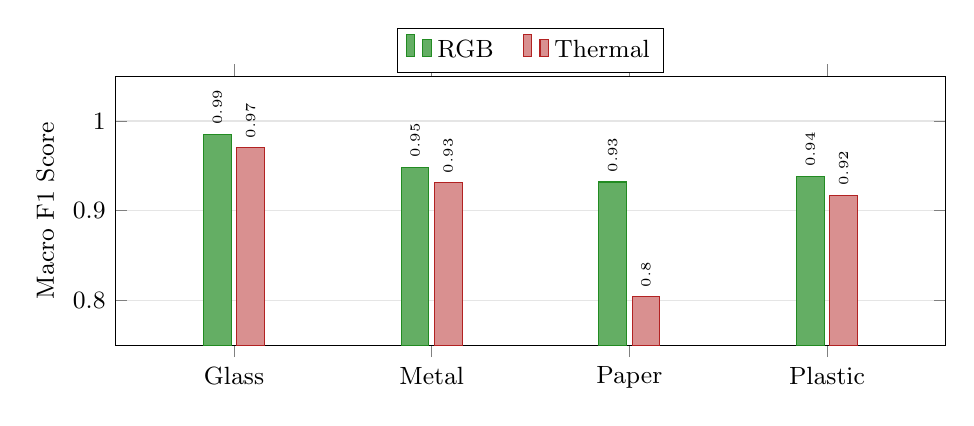
\begin{tikzpicture}
\begin{axis}[
  ybar,
  bar width=10pt,
  width=\columnwidth,
  height=5cm,
  ylabel={Macro F1 Score},
  ylabel style={font=\small},
  symbolic x coords={Glass, Metal, Paper, Plastic},
  xtick=data,
  xticklabel style={font=\small},
  yticklabel style={font=\small},
  ymin=0.75, ymax=1.05,
  ymajorgrids=true,
  grid style={gray!20},
  legend style={
    at={(0.5, 1.18)},
    anchor=north,
    legend columns=2,
    font=\small,
    /tikz/every even column/.append style={column sep=0.3cm}
  },
  nodes near coords,
  every node near coord/.append style={font=\tiny, rotate=90, anchor=west},
  enlarge x limits=0.2,
]
\addplot[fill=rgbgreen!70, draw=rgbgreen] coordinates {
  (Glass, 0.985) (Metal, 0.948) (Paper, 0.932) (Plastic, 0.938)
};
\addplot[fill=thermalred!50, draw=thermalred] coordinates {
  (Glass, 0.970) (Metal, 0.931) (Paper, 0.804) (Plastic, 0.917)
};
\legend{RGB, Thermal}
\end{axis}
\end{tikzpicture}
\caption{Per-class F1 comparison: RGB vs.\ Thermal. RGB outperforms on all classes; largest gap on paper (0.932 vs.\ 0.804).}
\label{fig:comparison_chart}
\end{figure}

Figure~\ref{fig:comparison_chart} compares per-class F1 scores across both modalities. Key findings:

\begin{itemize}
  \item \textbf{RGB outperforms thermal overall} (95.1\% vs.\ 90.6\% macro F1), with both modalities achieving strong results using the same frozen DINOv2 backbone and identical trainable architecture.
  \item \textbf{Glass is near-perfect} in both pipelines (F1 $\geq$ 0.97), indicating highly distinctive visual and thermal signatures.
  \item \textbf{Paper is the hardest class} for both modalities, but especially for thermal (F1 = 0.804 vs.\ 0.932), reflecting inherently similar thermal signatures between paper and plastic.
  \item \textbf{Thermal shows higher variance} across folds ($\pm$0.04 vs.\ $\pm$0.01), suggesting that thermal features are more sensitive to the specific train/test partition.
  \item Despite lower standalone accuracy, the \textbf{thermal modality captures complementary} material properties (thermal conductivity, emissivity) that benefit a downstream late fusion approach.
\end{itemize}

\end{document}
